\chapter{Manuales de Usuario}
\label{chap:manuales}
\drop{E}{n} este anexo se encuentran los manuales de usuario para los diferentes roles que hagan uso de la solución desarrollada.

\section*{Manual de Usuario para el Administrador}
El administrador será el responsable de la gestión de la plataforma y el encargado de dar de baja y añadir nuevos administradores y docentes en la base de datos. Por tanto, deberá conocer de una manera adecuada los procedimientos a realizar en cada uno de los casos o tareas que deba desempeñar. Este usuario tendrá acceso al proyecto de Firebase, cuya página inicial se muestra en la Figura \ref{fig:iniciofirebase}.

\begin{figure}[!h]
	\begin{center}
		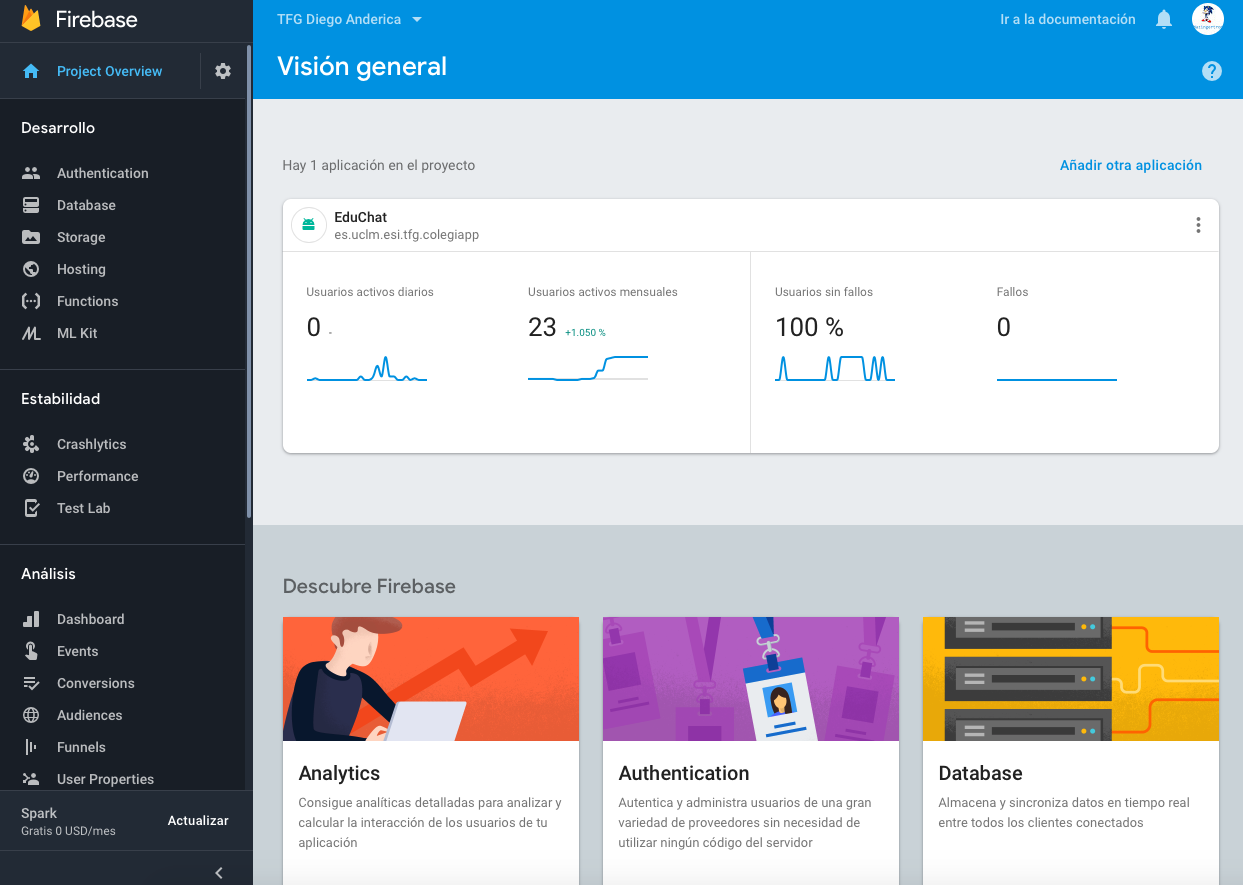
\includegraphics[width=0.95\textwidth]{/manuales/administrador/inicio_firebase}
		\caption{Página de Inicio del Proyecto de Firebase}
		\label{fig:iniciofirebase}
	\end{center}
\end{figure}

\clearpage

En la columna lateral izquierda se encuentran todas las funciones que puede ofrecer la plataforma de Google, aunque primero se hablará de \textit{Database}, que se trata de la base de datos no relacional donde se alojará la mayor parte de la información. Una vez que el administrador se haya dirigido a este apartado, se mostrará una página Web con la información de la base de datos organizada en colecciones (Figura \ref{fig:iniciobbdd}). A continuación, se explicará cómo añadir nuevos docentes, así como nuevos administradores.

\begin{figure}[!h]
	\begin{center}
		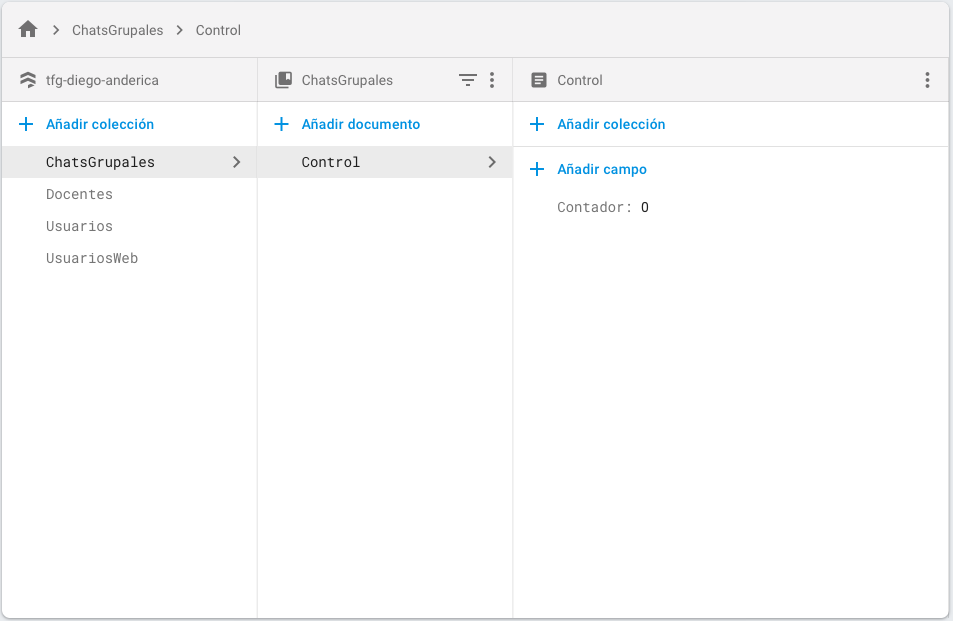
\includegraphics[width=0.95\textwidth]{/manuales/administrador/inicio_bbdd}
		\caption{Página de Inicio de la Base de Datos}
		\label{fig:iniciobbdd}
	\end{center}
\end{figure}

\clearpage

\subsection*{Añadir un Nuevo Docente}
En el caso de que un administrador desee dar de alta a un nuevo docente, bastará con dirigirse a la colección <<Docentes>>, haciendo clic sobre ella. El sitio Web mostrará todos los documentos existentes que representan a cada uno de los docentes registrados (Figura \ref{fig:bbdddocentes}). Posteriormente, deberá pulsar sobre el botón <<Añadir documento>>, que se encuentra situado en la columna central para comenzar el procedimiento. Se abrirá un nuevo formulario (Figura \ref{fig:adddocente}), donde el administrador podrá comenzar a rellenar los campos que se muestran en el ejemplo de la Figura \ref{fig:bbdddocentes} con la información del nuevo docente, haciendo clic sobre el botón <<Añadir campo>> para introducir nuevos campos. El tipo en todos los campos deberá ser \textit{String}.

\begin{figure}[!h]
	\begin{center}
		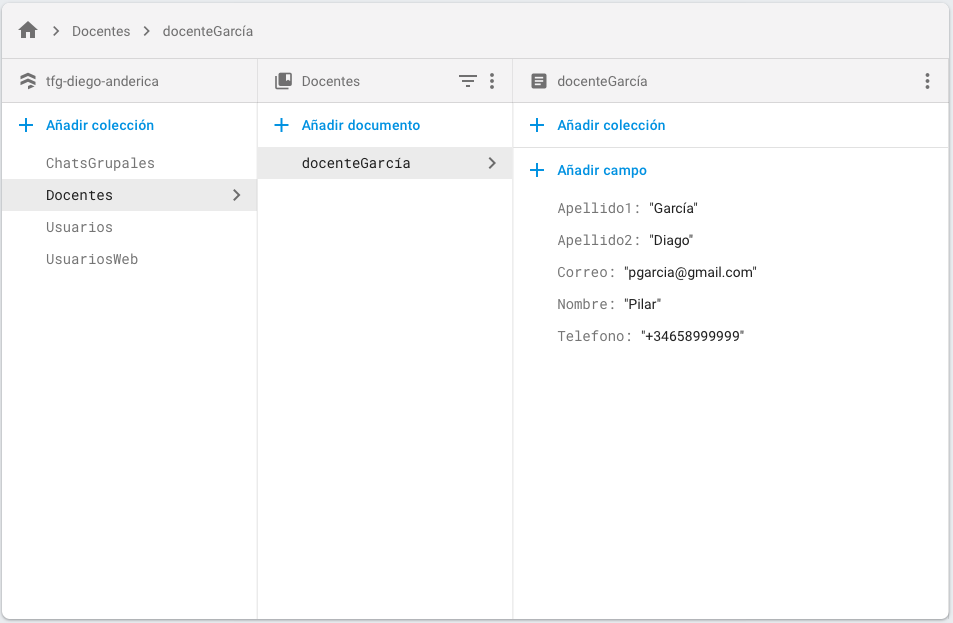
\includegraphics[width=0.7\textwidth]{/manuales/administrador/bbdd_docentes}
		\caption{Ejemplo Colección Docentes}
		\label{fig:bbdddocentes}
	\end{center}
\end{figure}

\begin{figure}[!h]
	\begin{center}
		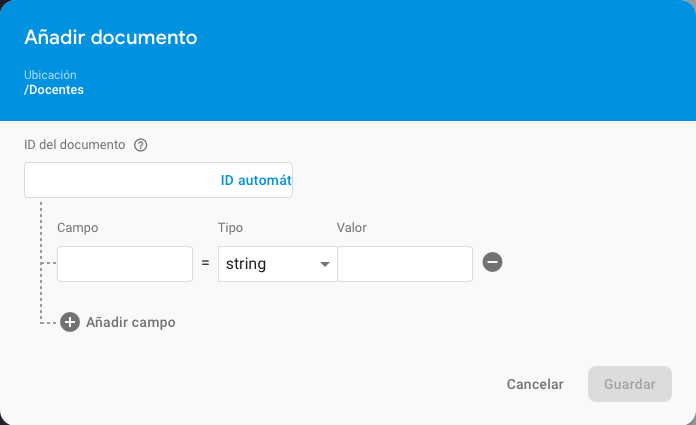
\includegraphics[width=0.7\textwidth]{/manuales/administrador/add_docente}
		\caption{Añadir Nuevo Documento}
		\label{fig:adddocente}
	\end{center}
\end{figure}

\clearpage

Un ejemplo en el que se añadiría un nuevo docente es el que se muestra en la Figura \ref{fig:errordocente}, donde el campo <<ID del documento>> deberá rellenarse (sin tildes para una mayor consistencia) con la estructura \mbox{\textit{docentePrimerApellidoX}}, siendo X un número, en caso de que ya exista otro docente con el mismo identificador, situación que será advertida (Figura \ref{fig:errordocente}).

\begin{figure}[!h]
	\begin{center}
		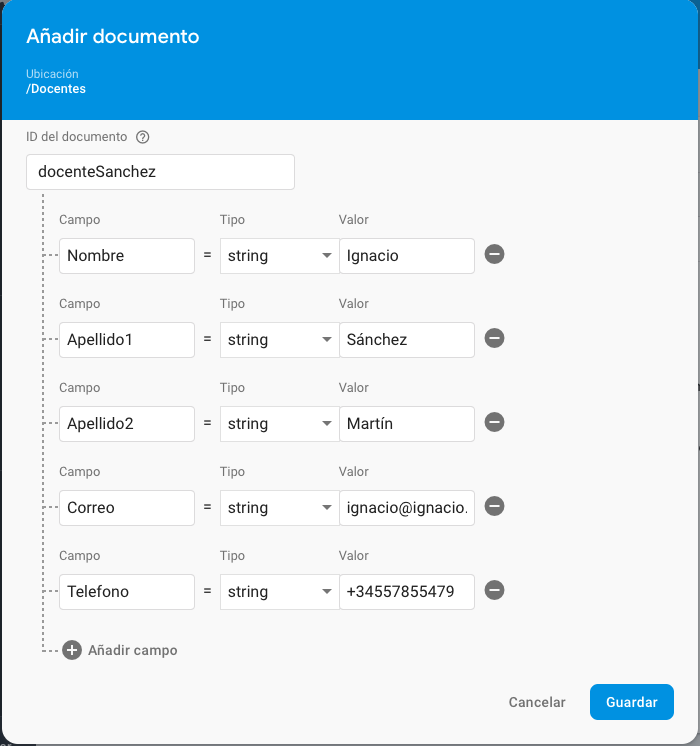
\includegraphics[width=0.7\textwidth]{/manuales/administrador/ejemplodocente}
		\caption{Ejemplo de Creación de un Nuevo Docente}
		\label{fig:ejemploocente}
	\end{center}
\end{figure}

\begin{figure}[!h]
	\begin{center}
		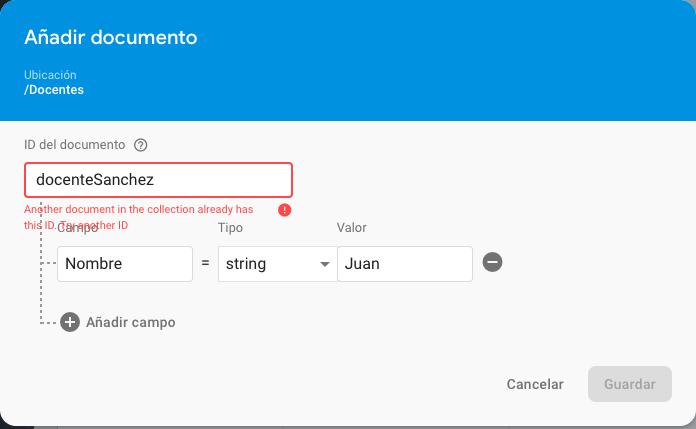
\includegraphics[width=0.7\textwidth]{/manuales/administrador/errordocente}
		\caption{Documento Existente}
		\label{fig:errordocente}
	\end{center}
\end{figure}

Una vez finalizado el proceso, se debe hacer clic en el botón <<Guardar>>, situado en el borde inferior derecho, quedando registrado el nuevo docente en la base de datos (Figura \ref{fig:finadddocente}).

\begin{figure}[!h]
	\begin{center}
		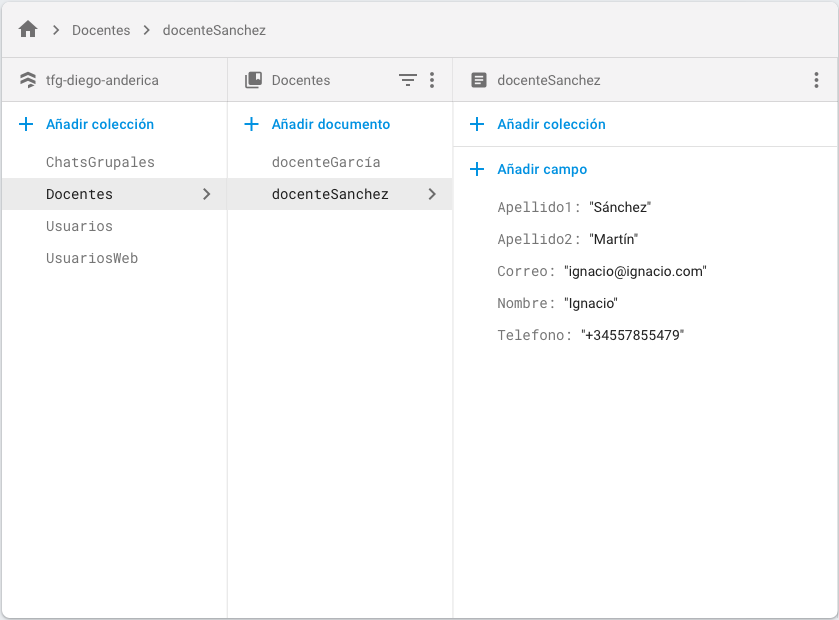
\includegraphics[width=0.75\textwidth]{/manuales/administrador/finadd_docente}
		\caption{Alta de Nuevo Docente Finalizada}
		\label{fig:finadddocente}
	\end{center}
\end{figure}

\subsection*{Eliminar un Docente}
Al igual que se pueden registrar nuevos docentes, también es posible eliminarlos de la base de datos. Para ello, una vez en vista de la colección <<Docentes>>, si se tuviera demasiados docentes para realizar una búsqueda manual, Firebase proporciona un filtro, representado mediante un botón con tres líneas horizontales (Figura \ref{fig:filtrodocente}) para buscar documentos por cada uno de los campos, es decir, <<Nombre>>, <<Apellido1>>, <<Telefono>>, etc.

\begin{figure}[!h]
	\begin{center}
		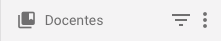
\includegraphics[width=0.4\textwidth]{/manuales/administrador/filtrodocente}
		\caption{Botón para Establecer un Filtro}
		\label{fig:filtrodocente}
	\end{center}
\end{figure}

\clearpage

Una vez que se haya encontrado el documento correspondiente al docente que se desea eliminar, bastará con seleccionarlo y abrir el menú que se encuentra en la tercera columna, haciendo clic sobre el botón con tres puntos alineados verticalmente y seleccionar la opción <<Eliminar documento>> (Figura \ref{fig:eliminardocente}). La página Web avisará de que se desea borrar ese documento y, una vez confirmada la acción, el docente será eliminado definitivamente de la base de datos

\begin{figure}[!h]
	\begin{center}
		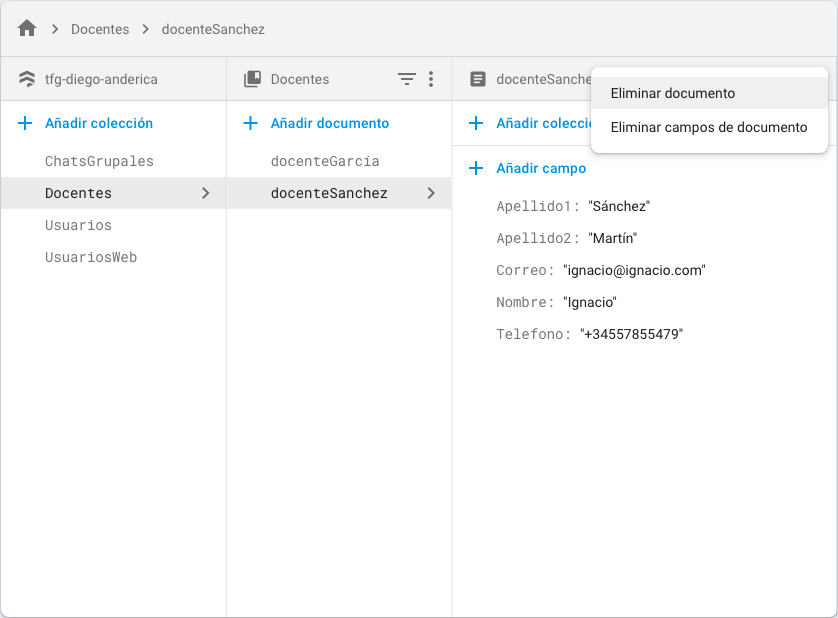
\includegraphics[width=0.7\textwidth]{/manuales/administrador/eliminardocente}
		\caption{Eliminar Docente}
		\label{fig:eliminardocente}
	\end{center}
\end{figure}

\clearpage

\subsection*{Añadir un Nuevo Administrador}
Los administradores también tendrán la capacidad de añadir nuevos administradores mediante la página Web de Firebase. Para ello, se deberá dirigir a la colección <<UsuariosWeb>> de la base de datos, donde se encontrarán todos los administradores actuales (Figura \ref{fig:bbdduweb}). En este caso, cada uno de los documentos tendrán únicamente dos campos: <<Correo>> y <<Contrasena>>, que son los datos requeridos para iniciar sesión en la página Web de administración.

\begin{figure}[!h]
	\begin{center}
		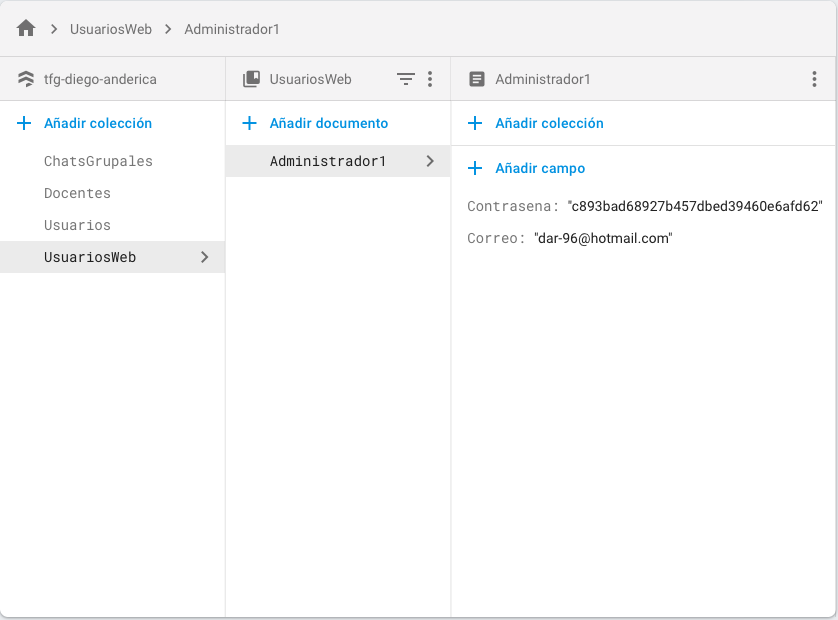
\includegraphics[width=0.7\textwidth]{/manuales/administrador/bbdd_admins}
		\caption{Colección <<UsuariosWeb>>}
		\label{fig:bbdduweb}
	\end{center}
\end{figure}

Los pasos a realizar para dar de alta a un administrador son muy similares a los que se deben seguir para dar de alta a un docente: se pulsa el botón <<Añadir documento>>, se rellenan los datos correspondientes y se pulsa el botón <<Guardar>>. En este caso, el <<ID del documento>> tendrá el formato \mbox{\textit{AdministradorX}}, siendo X un número que no se repita en la base de datos. Los datos serán proporcionados por el administrador entrante, puesto que es el único conocedor del campo <<Contrasena>>.

\subsection*{Eliminar un Administrador}
De igual manera a lo que se muestra en la Figura \ref{fig:eliminardocente}, se deberá seleccionar el documento del administrador a eliminar, pulsar sobre el botón de la tercera columna con tres puntos alineados verticalmente y seleccionar la opción <<Eliminar documento>>. De esta manera, se habrá eliminado un administrador de la base de datos.

\clearpage

\subsection*{Uso de la Página Web de Gestión}
Los administradores serán también los encargados de gestionar las familias en la base de datos, aunque esta tarea se puede realizar de una manera más cómoda desde la página Web que se ha diseñado con ese fin. Lo primero que se muestra al intentar acceder es una página de inicio de sesión (Figura \ref{fig:loginweb}), donde se deberán introducir el correo electrónico y la contraseña del administrador que, previamente, ha de estar registrado en la base de datos.

\begin{figure}[!h]
	\begin{center}
		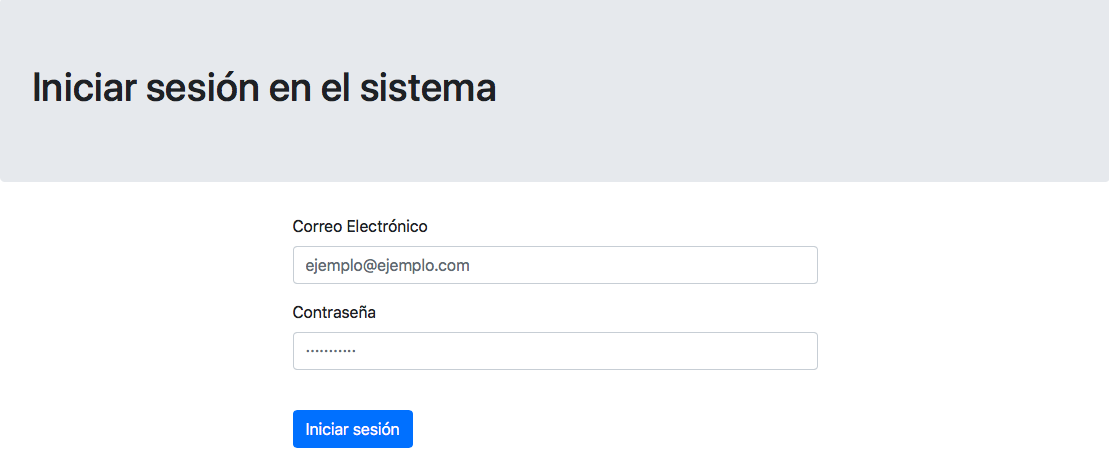
\includegraphics[width=0.8\textwidth]{/manuales/administrador/loginweb}
		\caption{Página de Inicio de Sesión}
		\label{fig:loginweb}
	\end{center}
\end{figure}

Una vez que el administrador se ha identificado correctamente, se puede comenzar a gestionar usuarios mediante una de las opciones que se muestran en la página principal: dar de alta, dar de baja, consultar o modificar usuarios (Figura \ref{fig:indexweb}). Todas estas opciones estarán disponibles de igual manera a través de la barra superior, desde donde se podrá, además, navegar hacia la página inicial haciendo clic sobre <<Gestión de Usuarios>> o cerrar la sesión mediante el botón con el mismo nombre situado en la esquina superior derecha. De aquí en adelante se explicarán cada una de las funciones principales que ofrece la página Web.

\begin{figure}[!h]
	\begin{center}
		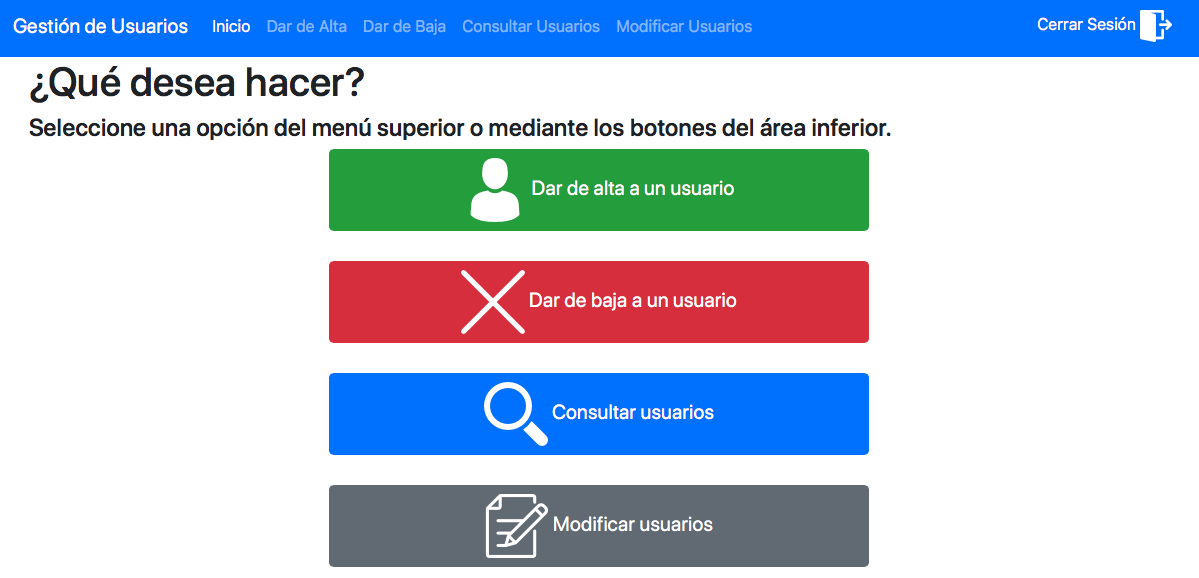
\includegraphics[width=0.8\textwidth]{/manuales/administrador/mainweb}
		\caption{Página Principal}
		\label{fig:indexweb}
	\end{center}
\end{figure}

\clearpage

\subsubsection*{Dar de Alta}
Al entrar en la página para dar de alta a nuevos usuarios, se tiene la posibilidad de hacerlo mediante la subida de un archivo o rellenando manualmente cada uno de los campos. Si se desea dar de alta usando un archivo con extensión \acs{CSV}, se deberá seleccionar mediante el botón <<Seleccionar archivo>> y, una vez hecho esto, pulsar sobre <<Subir Archivo>>. El navegador comenzará a realizar el registro de los usuarios en la base de datos y se notificará cuando la operación se haya completado.

Por otra parte, si se desea rellenar el formulario, se deberán especificar los campos que se encuentran disponibles. Si la familia posee dos tutores legales, se deberán habilitar los campos del segundo tutor legal pulsando sobre el botón <<Habilitar Campos Tutor 2>> (Figura \ref{fig:altaweb}). Por el contrario, si la familia únicamente posee un tutor legal, se deberán deshabilitar dichos campos pulsando sobre el mismo botón. Una vez que se tengan todos los datos introducidos, se puede pulsar sobre el botón <<Generar Nombre de Familia>> para observar en el campo <<Nombre de la familia>> con qué identificador se registrará de manera única en la base de datos, puesto que podría ser útil a la hora de realizar una consulta, aunque no es necesaria su generación por parte del administrador. En caso de que se pulse sobre el botón <<Dar de Alta Usuario/Familia>> sin haber generado su identificador, se generará automáticamente.

\begin{figure}[!h]
	\begin{center}
		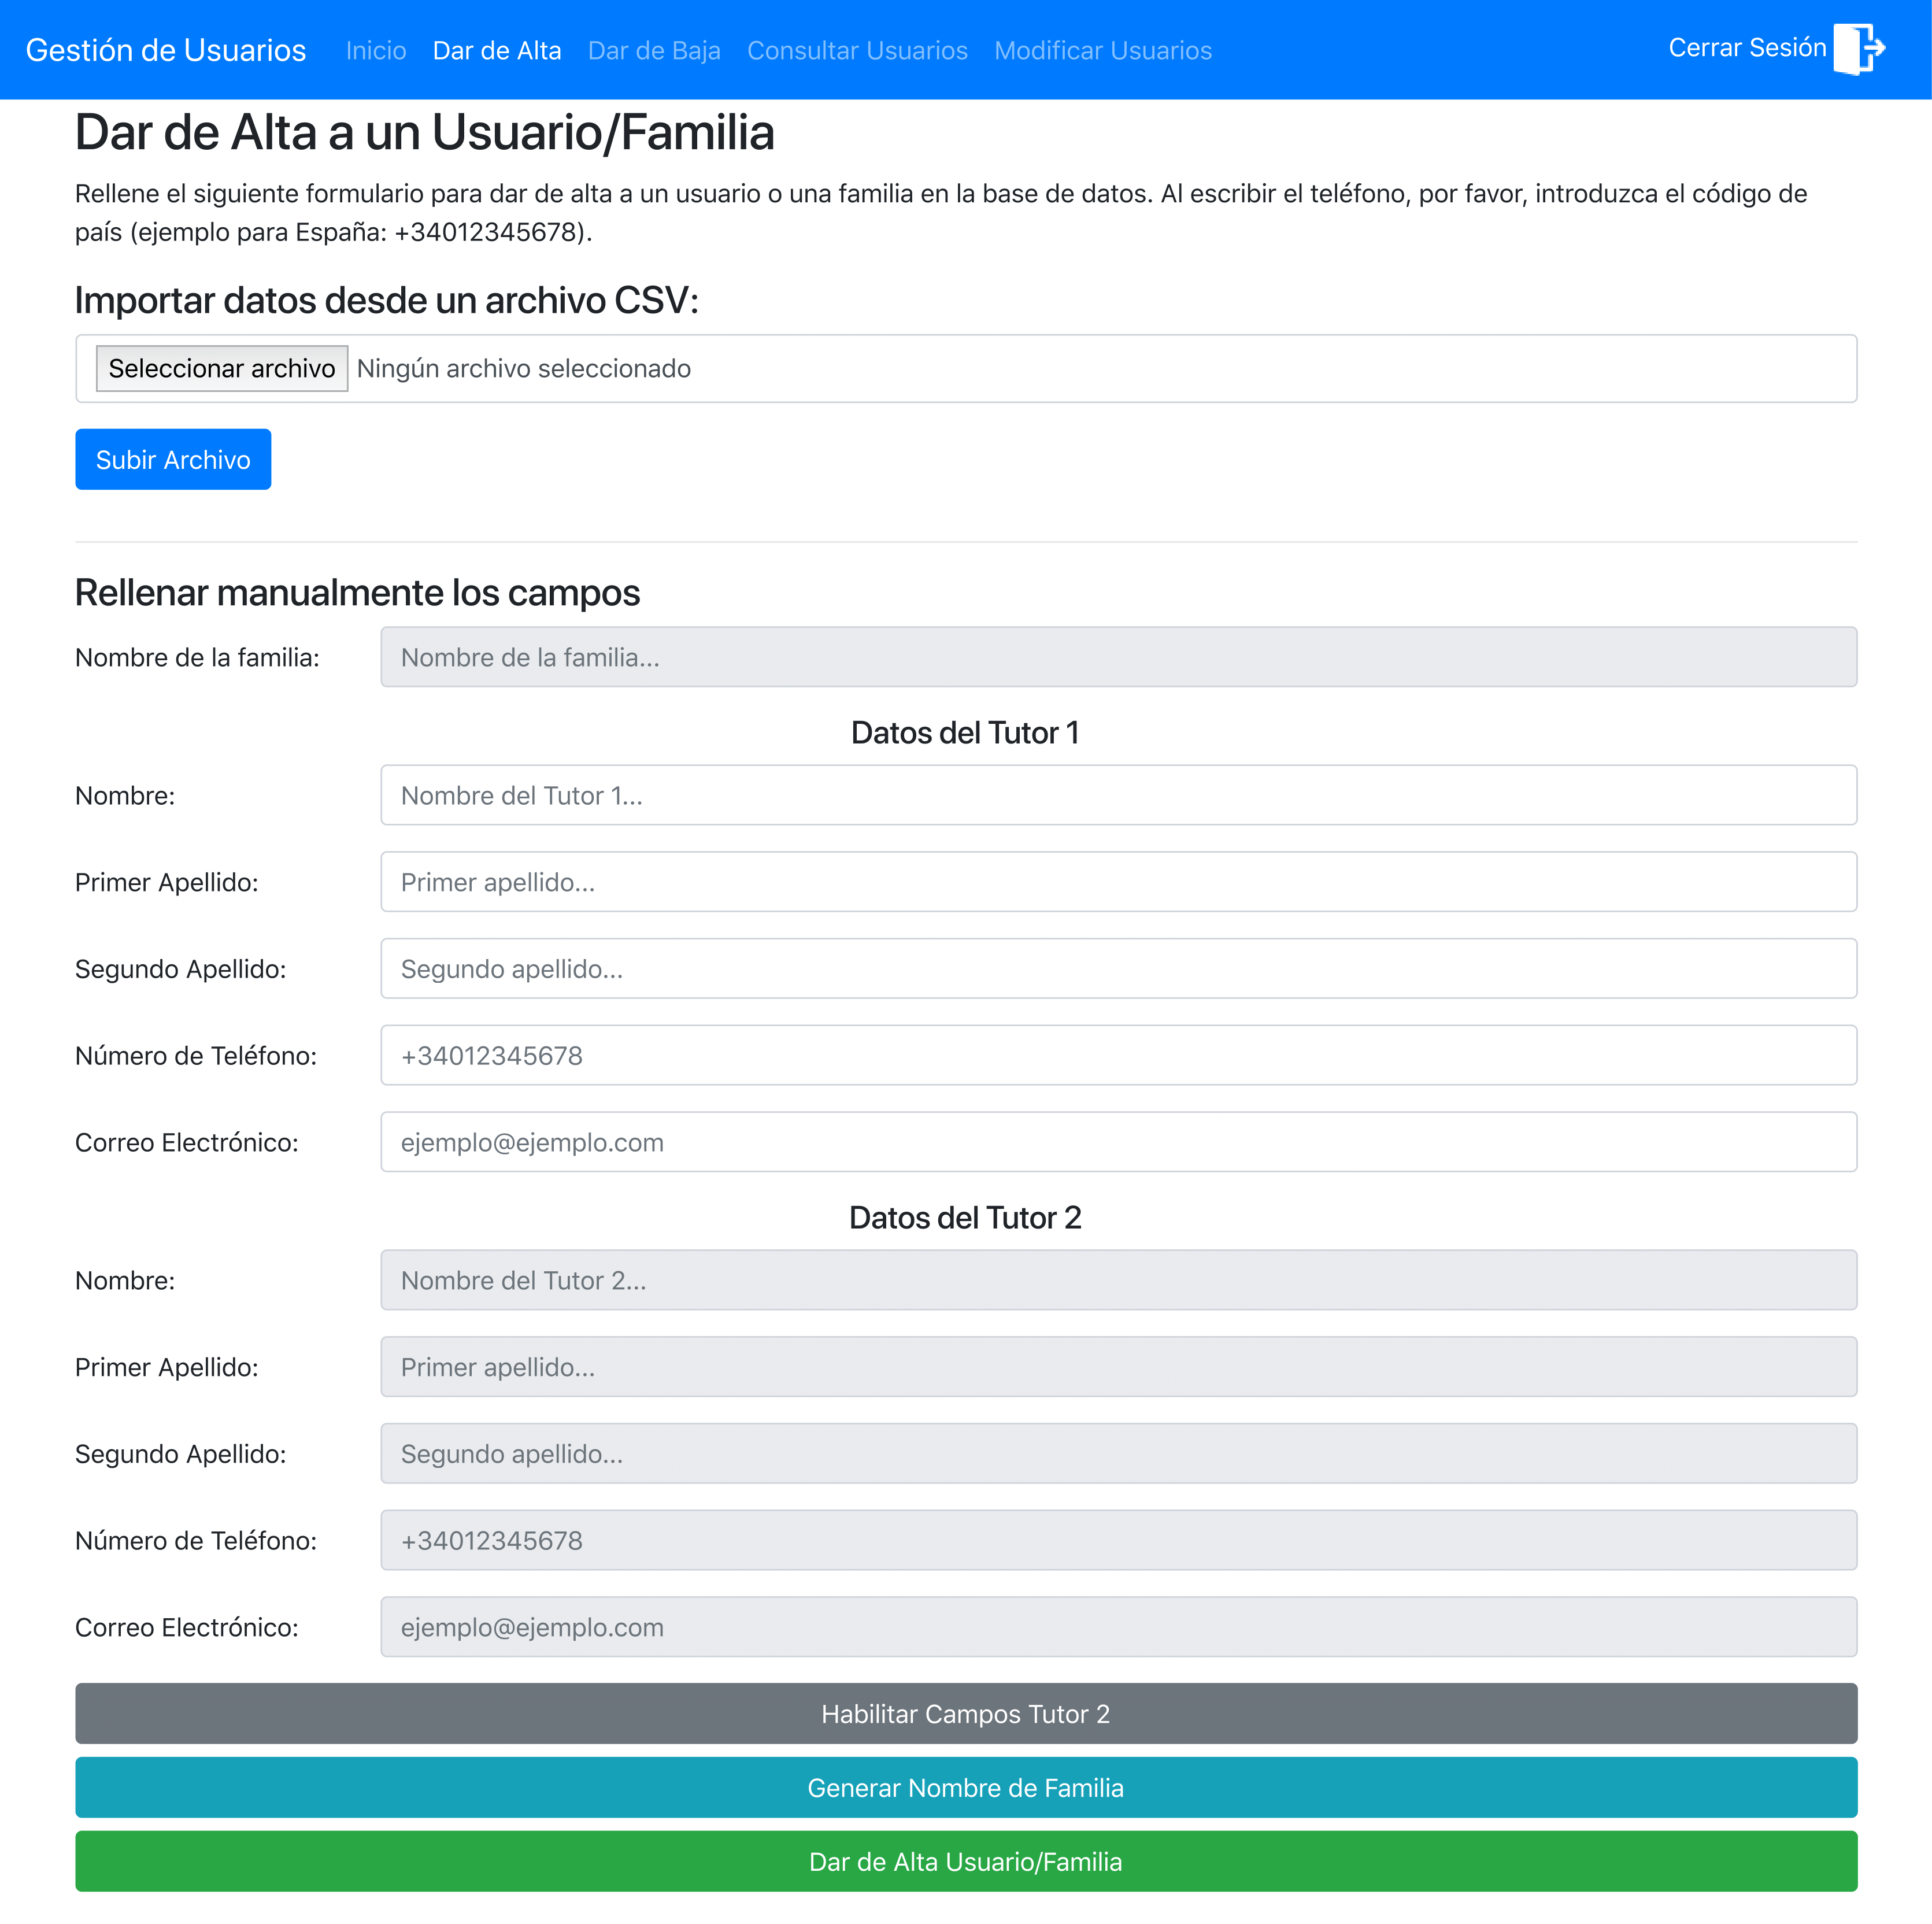
\includegraphics[width=0.75\textwidth]{/manuales/administrador/alta}
		\caption{Página para Dar de Alta a Nuevos Usuarios}
		\label{fig:altaweb}
	\end{center}
\end{figure}

\clearpage

\subsubsection*{Dar de Baja}
La página para dar de baja a una familia muestra una lista desplegable con una tabla. En dicha lista se encontrarán todos los identificadores de las familias registradas en la base de datos. Al seleccionar uno de ellos, se rellena la tabla con los datos y, al pulsar sobre el botón <<Dar de Baja Usuario/Familia>>, se eliminará la familia seleccionada de la base de datos (Figura \ref{fig:bajaweb}).

\begin{figure}[!h]
	\begin{center}
		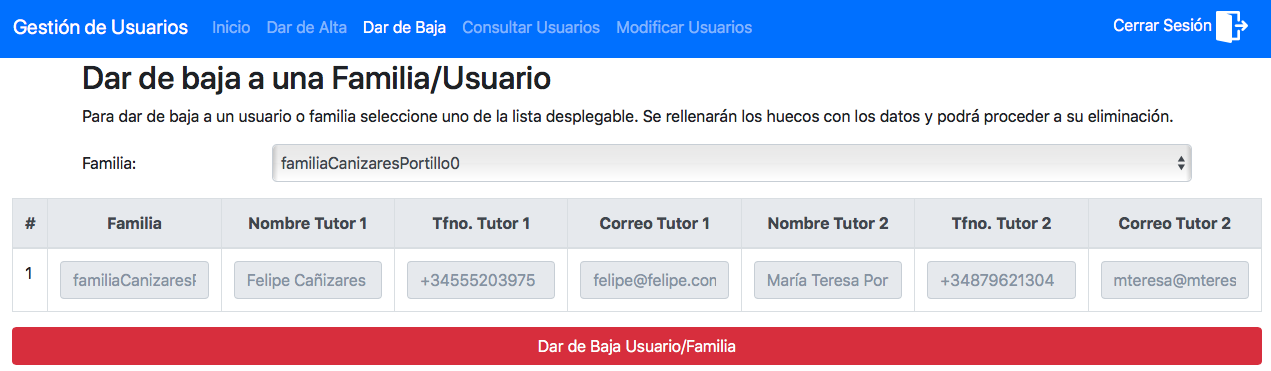
\includegraphics[width=0.8\textwidth]{/manuales/administrador/bajafamilia}
		\caption{Página de Baja de Familias}
		\label{fig:bajaweb}
	\end{center}
\end{figure}

\subsubsection*{Consultar Usuarios}
La página Web de gestión también permite realizar consultas acerca de las familias que se encuentran registradas. Para ello, en el apartado correspondiente de la misma, se ofrece un filtro para buscar de acuerdo a los diferentes campos. Es decir, se puede introducir un <<texto a buscar>> y seleccionar sobre qué campo se quiere hacer la consulta mediante la lista desplegable. En el caso de que se quiera ver de un vistazo todas las familias registradas en la base de datos, se deberá dejar el campo de <<texto a buscar>> en blanco y pulsar sobre el botón <<Buscar>> (Figura \ref{fig:consultaweb}).

\begin{figure}[!h]
	\begin{center}
		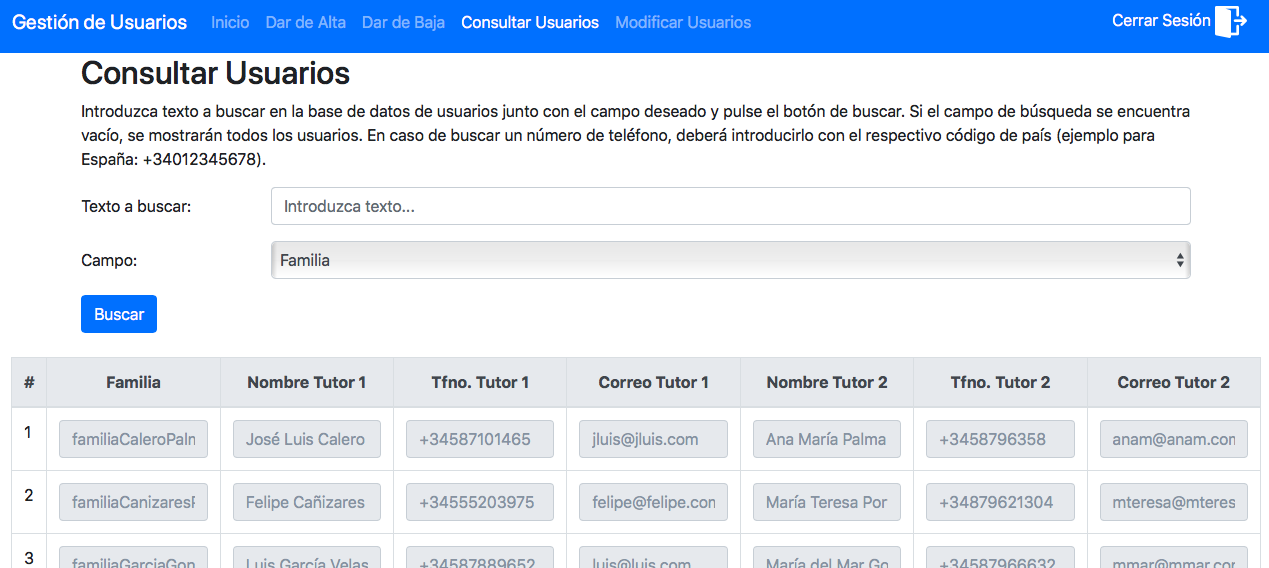
\includegraphics[width=0.85\textwidth]{/manuales/administrador/consulta}
		\caption{Página de Consulta}
		\label{fig:consultaweb}
	\end{center}
\end{figure}

\clearpage

\subsubsection*{Modificar Usuarios}
Por último, la funcionalidad de modificar usuarios permite cambiar los datos de las familias que están registradas en la base de datos sin la necesidad de eliminar por completo el registro y crearlo de nuevo. Al acceder a la página se muestra una lista desplegable con todos los registros y, seleccionando uno de ellos, se cargan automáticamente todos los datos asociados al mismo en los campos que se encuentran debajo de dicha lista de manera que se pueda visualizar previamente lo que se desea cambiar. Al pulsar el botón <<Modificar Usuario/Familia>> se habilitan todos los campos para su modificación. Una vez que se haya finalizado dicha modificación de datos, se deberá hacer clic sobre el botón anterior, que ahora mostrará <<Confirmar Modificación>> o, si se desea anular el proceso, se hará clic sobre el botón rojo <<Cancelar>>, volviendo a bloquear todos los campos y no afectando ningún cambio en la base de datos (Figura \ref{fig:modificarweb}).

\begin{figure}[!h]
	\begin{center}
		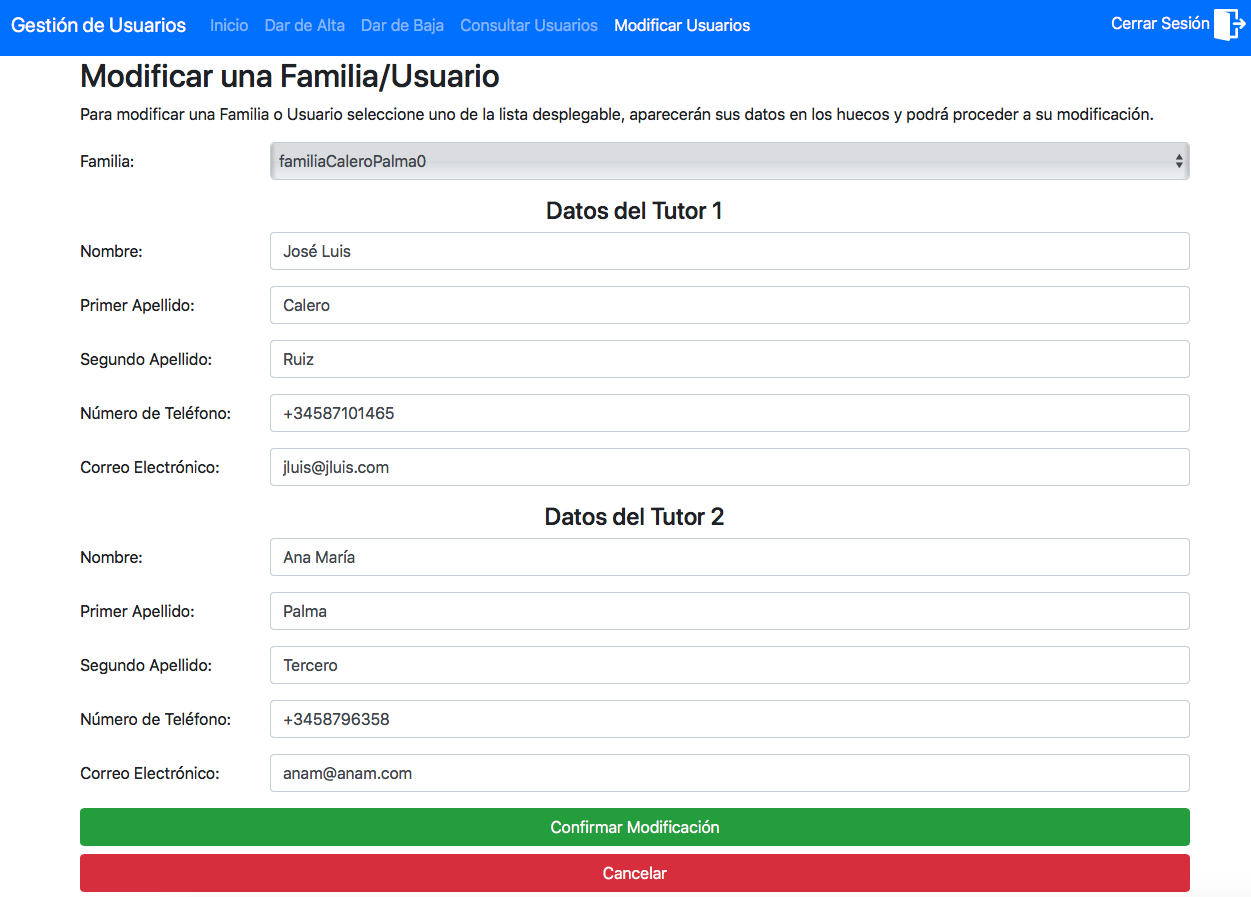
\includegraphics[width=0.85\textwidth]{/manuales/administrador/modificar}
		\caption{Página de Modificación de Usuarios}
		\label{fig:modificarweb}
	\end{center}
\end{figure}

\clearpage

\section*{Manual de Usuario para Docentes}
Los docentes serán los que tendrán la responsabilidad de crear y mantener los diferentes chats que puedan existir en la aplicación móvil. Por tanto, es relevante que se conozca el funcionamiento de la misma, a fin de llevar a cabo dicha tarea de una manera adecuada.

\subsection*{Iniciar Sesión}
Lo primero que muestra la aplicación la primera vez que se utiliza en un \textit{smartphone} es la pantalla de bienvenida, donde se inicia el procedimiento de identificación e inicio de sesión del usuario (Figura \ref{fig:inicioappdocente}). En esta pantalla se muestran tres botones, siendo los dos primeros dedicados a los usuarios de las familias, mientras que el último (<<Soy Docente>>), está dedicado específicamente al inicio de sesión por parte de los docentes registrados. Al pulsar, se mostrará un diálogo preguntando si se desea acceder mediante correo electrónico y contraseña o usando el número de teléfono asociado al docente (Figura \ref{fig:preguntadocente}).

\begin{figure}[!h]
	\centering
	\begin{minipage}{.5\textwidth}
		\centering
		\includegraphics[width=0.6\textwidth]{/manuales/docente/inicioapp}
		\caption{Pantalla de Inicio de EduChat}
		\label{fig:inicioappdocente}
	\end{minipage}%
	\begin{minipage}{.5\textwidth}
		\centering
		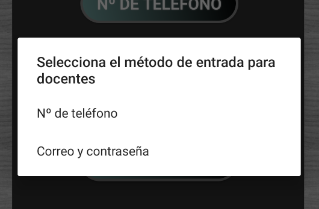
\includegraphics[width=0.8\textwidth]{manuales/docente/preguntadocente}
		\caption{Pregunta de Inicio de Sesión}
		\label{fig:preguntadocente}
	\end{minipage}
\end{figure}

\clearpage

En el caso en el que se elija iniciar sesión mediante el número de teléfono, se mostrará una actividad en la que se deberá introducir el número de teléfono y pulsar el botón <<Enviar Código>> (Figura \ref{fig:iniciotfnodocente}). Unos instantes después se recibirá un \acs{SMS} con un código que se deberá introducir en la aplicación para poder finalizar el inicio de sesión. Por el contrario, si se desea iniciar sesión haciendo uso del correo electrónico y una contraseña, el docente deberá introducir ambos valores en la pantalla que se muestra (Figura \ref{fig:iniciocorreodocente}). Si es la primera vez que se inicia sesión, la contraseña que se introduzca será la que quede registrada en la base de datos. No obstante, existe la posibilidad de cambiarla en caso de que así se desee o se haya olvidado mediante la opción <<¿Has olvidado tu contraseña?>>, en cuyo caso se deberá introducir el correo electrónico y pulsar el botón de <<Enviar Correo>> para recibir un mensaje en la dirección escrita. Dicho mensaje contendrá un enlace con instrucciones a seguir para cambiar la contraseña de acceso.

\begin{figure}[!h]
	\centering
	\begin{minipage}{.5\textwidth}
		\centering
		\includegraphics[width=0.6\textwidth]{/manuales/docente/iniciotfno}
		\caption{Pantalla de Inicio con Número \\ de Tfno.}
		\label{fig:iniciotfnodocente}
	\end{minipage}%
	\begin{minipage}{.5\textwidth}
		\centering
		\includegraphics[width=0.6\textwidth]{manuales/docente/iniciocorreo}
		\caption{Pantalla de Inicio con Correo y Contraseña}
		\label{fig:iniciocorreodocente}
	\end{minipage}
\end{figure}

\clearpage

\subsection*{Crear un Nuevo Chat}
Una vez que se ha iniciado sesión y se ha accedido a la aplicación, el docente podrá crear nuevos chats mediante el menú situado en la esquina superior derecha, representado con tres puntos alineados verticalmente, seleccionando la opción <<Crear nuevo chat...>>. A continuación, deberá escoger un nombre para el nuevo chat, así como los integrantes que conformarán el mismo (Figura \ref{fig:crearchat}). Una vez hecho esto, se finalizará la creación pulsando el botón <<Crear Chat>>. Este nuevo chat se mostrará en la pantalla principal de la aplicación, así como cualquier otro del que se sea miembro. Además, los docentes podrán eliminar los chats que hayan creado, realizando una pulsación larga sobre su nombre en la lista de la pantalla principal, tras lo que se mostrará un diálogo confirmando la eliminación. (Figura \ref{fig:eliminarchat}).

\begin{figure}[!h]
	\centering
	\begin{minipage}{.5\textwidth}
		\centering
		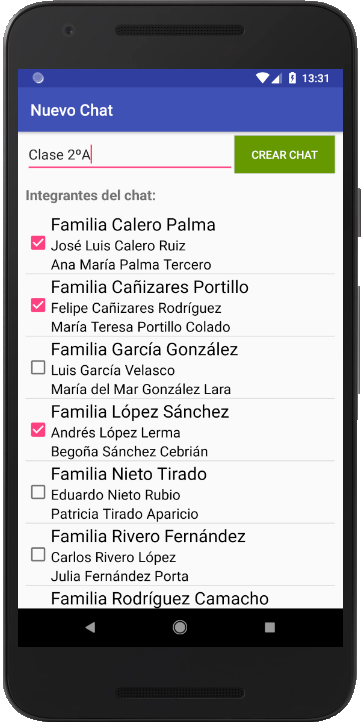
\includegraphics[width=0.6\textwidth]{/manuales/docente/crearchat}
		\caption{Pantalla de Creación de Chat}
		\label{fig:crearchat}
	\end{minipage}%
	\begin{minipage}{.5\textwidth}
		\centering
		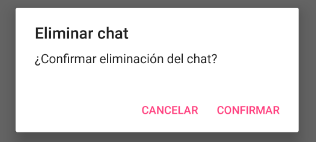
\includegraphics[width=0.8\textwidth]{manuales/docente/eliminar}
		\caption{Confirmación de Borrado de Chat}
		\label{fig:eliminarchat}
	\end{minipage}
\end{figure}

\clearpage

\subsection*{Ver Perfil y Cambiar Imagen}
Mediante el menú principal de la aplicación también se permite visualizar la información del usuario, así como la imagen de perfil, si tuviera una definida (Figura \ref{fig:perfildocente}). Si se desea establecer una nueva imagen, se podrá hacer mediante el botón <<Cambiar Imagen de Perfil>>, pudiendo escoger alguna fotografía de la galería. Por el contrario, si se desea eliminar la imagen de perfil, se podrá realizar pulsando el botón <<Eliminar Imagen de Perfil>>, restableciendo el avatar por defecto.

\begin{figure}[!h]
	\begin{center}
		\includegraphics[width=0.4\textwidth]{/manuales/docente/perfil}
		\caption{Pantalla de Perfil}
		\label{fig:perfildocente}
	\end{center}
\end{figure}

\clearpage

\subsection*{Ver Información de Grupo}
Todos los grupos poseen un apartado en el que se muestra su información. Se puede acceder mediante el botón <<Info.>>, que se encuentra en la esquina superior derecha. Desde esta pantalla se puede visualizar el nombre del grupo, así como los integrantes de este (Figura \ref{fig:infochatdocente}). Asimismo, se puede visualizar al lado de cada integrante un número en forma de porcentaje, que representa el tono que ha tenido este en el chat, siendo 0\% el peor resultado y el 100\% el mejor. De igual manera, se podrá visualizar el tono individual de cada mensaje con colores rojo, naranja, amarillo y verde, en orden creciente de puntuación. Además se podrá acceder a la información de cada familia pulsando sobre el nombre de estas (Figura \ref{fig:infointegrantedocente}).

\begin{figure}[!h]
	\centering
	\begin{minipage}{.5\textwidth}
		\centering
		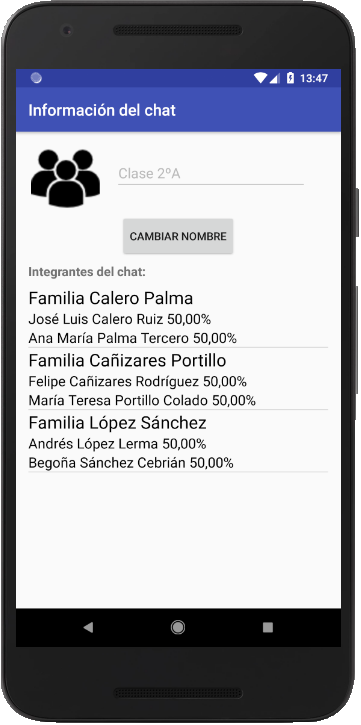
\includegraphics[width=0.6\textwidth]{/manuales/docente/infochat}
		\caption{Pantalla de Información \\ del Chat}
		\label{fig:infochatdocente}
	\end{minipage}%
	\begin{minipage}{.5\textwidth}
		\centering
		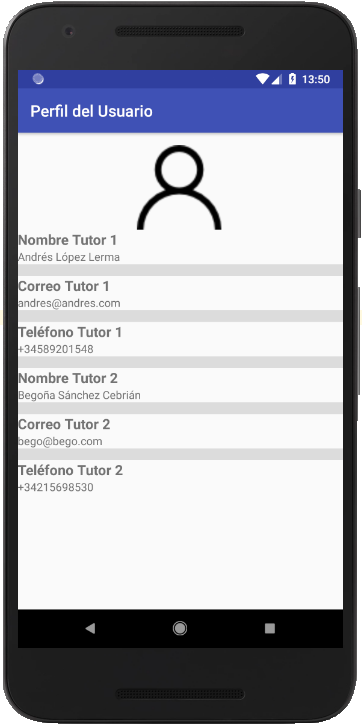
\includegraphics[width=0.6\textwidth]{manuales/docente/infointegrante}
		\caption{Pantalla de Información de \\ Integrante}
		\label{fig:infointegrantedocente}
	\end{minipage}
\end{figure}

\clearpage

\subsection*{Crear Eventos de Calendario}
Un docente puede crear un evento de calendario para avisar a los integrantes del chat de acontecimientos futuros, tales como reuniones, charlas, excursiones, etc. Para ello, bastará pulsar sobre el botón (+) que se encuentra en la esquina inferior izquierda (Figura \ref{fig:creareventodocente}), lanzando la aplicación de calendario con todos los correos electrónicos de los integrantes del chat. Únicamente se debe especificar el nombre del evento, duración o lugar para completar la información de este y que sea de mayor utilidad para los invitados al mismo.

\begin{figure}[!h]
	\begin{center}
		
\includegraphics[width=0.3\textwidth]{/manuales/docente/crearevento}
		\caption{Botón para Crear Evento}
		\label{fig:creareventodocente}
	\end{center}
\end{figure}

\clearpage

\section*{Manual de Usuario para las Familias}
A continuación, se detallará el uso de la aplicación móvil, así como las funcionalidades principales para los usuarios de las familias registradas.

\subsection*{Iniciar Sesión}
La primera vez que se ejecuta la aplicación se debe iniciar sesión usando número de teléfono o correo electrónico y contraseña, métodos que se encuentran disponibles mediante dos botones en la pantalla inicial (Figura \ref{fig:inicioappfamilia}), reservándose el último botón <<Soy Docente>> para los docentes del centro.

\begin{figure}[!h]
	\begin{center}
		\includegraphics[width=0.4\textwidth]{/manuales/familia/inicioapp}
		\caption{Pantalla Inicio de la Aplicación}
		\label{fig:inicioappfamilia}
	\end{center}
\end{figure}

\clearpage

Si se selecciona iniciar sesión mediante número de teléfono, se deberá introducir este en la aplicación y pulsar el botón <<Enviar Código>> (Figura \ref{fig:iniciotfnofamilia}). Acto seguido, se recibirá en el terminal un mensaje \acs{SMS} con un código que se deberá introducir para completar el inicio de sesión. Por el contrario, si se selecciona el método de entrada mediante correo y contraseña, se deberán introducir ambos parámetros y pulsar el botón <<Enviar>> (Figura \ref{fig:iniciocorreofamilia}). Si es la primera vez que se inicia sesión en la aplicación, la contraseña que se introduzca en el campo correspondiente será la que se use para futuros inicios de sesión. No obstante, esta contraseña se puede cambiar haciendo uso de la opción <<¿Has olvidado tu contraseña?>>. En este caso, se deberá introducir el correo electrónico al que se desea que se mande el mensaje de recuperación con las instrucciones necesarias. Principalmente, este mensaje consta de un enlace que se deberá seguir para introducir la nueva contraseña.

\begin{figure}[!h]
	\centering
	\begin{minipage}{.5\textwidth}
		\centering
		\includegraphics[width=0.6\textwidth]{/manuales/familia/iniciotfno}
		\caption{Pantalla de Inicio de Sesión \\ Mediante Nº de Teléfono}
		\label{fig:iniciotfnofamilia}
	\end{minipage}%
	\begin{minipage}{.5\textwidth}
		\centering
		\includegraphics[width=0.6\textwidth]{manuales/familia/iniciocorreo}
		\caption{Pantalla de Inicio de Sesión \\ Mediante Correo y Contraseña}
		\label{fig:iniciocorreofamilia}
	\end{minipage}
\end{figure}

\clearpage

\subsection*{Ver y Editar Perfil}
Una vez que se ha accedido a la aplicación, se puede visualizar la información registrada acerca de la familia. Para ello, se debe pulsar la opción <<Perfil...>>, situada en el menú principal de la aplicación que se encuentra en la esquina superior derecha, representado por tres puntos en posición vertical. Una vez dentro, se podrá, además, establecer una imagen personalizada para la familia o eliminarla y restablecer la imagen por defecto usando los botones <<Cambiar Imagen de Perfil>> y <<Eliminar Imagen de Perfil>>, respectivamente (Figura \ref{fig:perfilfamilia}).

\begin{figure}[!h]
	\begin{center}
		\includegraphics[width=0.4\textwidth]{/manuales/familia/perfil}
		\caption{Pantalla de Perfil}
		\label{fig:perfilfamilia}
	\end{center}
\end{figure}

\clearpage

\subsection*{Ver y Enviar Mensajes}
Los usuarios de las familias podrán ver los chats a los que han sido añadidos, no pudiendo crear nuevos. Todos estos chats se mostrarán en la pantalla principal de la aplicación en forma de lista y, pulsando sobre cada uno de ellos, entrarán a los mismos y podrán enviar y recibir mensajes.

\subsection*{Ver Información del Chat}
Los usuarios de la aplicación tienen disponible un botón <<Info.>> en cada chat, desde donde se puede ver el nombre del grupo, así como las familias que lo integran (Figura \ref{fig:infochatfamilia}).

\begin{figure}[!h]
	\begin{center}
		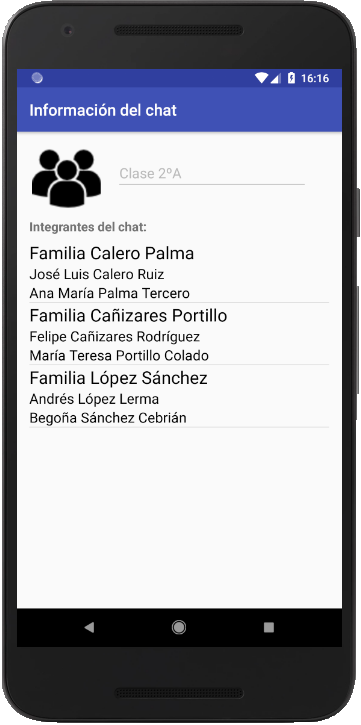
\includegraphics[width=0.4\textwidth]{/manuales/familia/infogrupo}
		\caption{Pantalla de Información de Chat}
		\label{fig:infochatfamilia}
	\end{center}
\end{figure}




